\section{Hyperparameter Tuning} \label{hpt}
For each model, the \textit{hyperparameters}, parameters that are not optimised by the training algorithm e.g. the number of trees in a random forest classifier, were tuned manually by using a grid search to test different values. A grid search uses brute force to search the entire space for different hyperparameter configurations. The best combination of hyperparameters for a model is determined by whichever has the highest accuracy on the validation set using 5-fold cross validation.

For logistic regression, the type of solver, penalty function and $C$ value were adjusted. \textit{Regularisation} prevents overfitting of training data by penalising large weights when training a logistic regression predictor, and the parameter $C$ mentioned is used to control the effect of this \cite{ahmadian1998regularisation}. The lower the value of $C$, the stronger the effect of regularisation. For the logistic regression model used in this paper, a $C$ value of 1.0, and a `liblinear' solver was chosen to give the best average accuracy score after hyperparameter tuning.

$l1$ regularisation penalises the sum of absolute values of weights, whereas $l2$ regularisation penalises the sum of squares of the weights \cite{ahmadian1998regularisation}. $l2$ regularisation was chosen and the learning curve of the logistic regression model can be seen in Figure \ref{lrlc}.

\begin{figure}[ht]
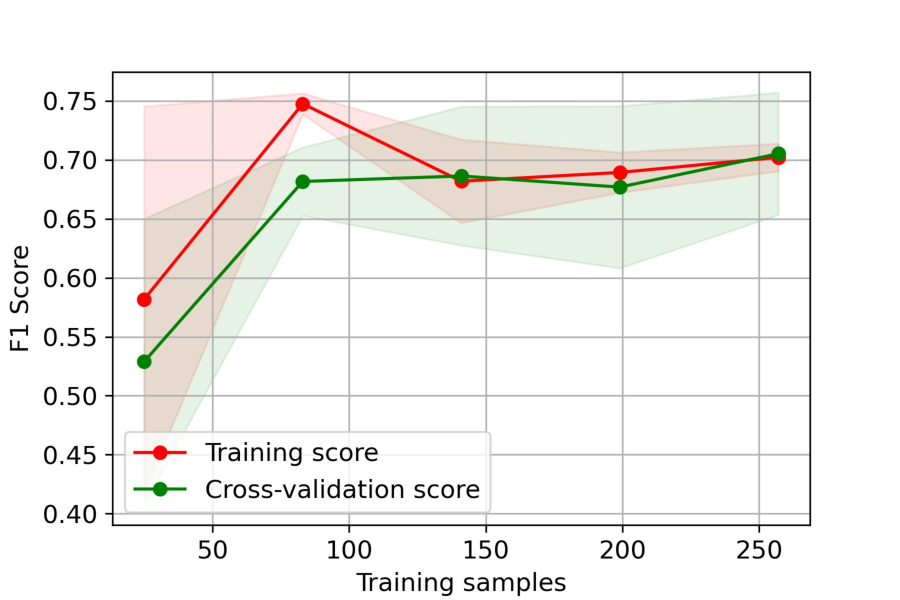
\includegraphics[width=8.5cm]{plots/LR TVT LC F1.pdf}
\caption{Logistic Regression Learning Curve}
\label{lrlc}
\centering
\end{figure}

\begin{figure}[t]
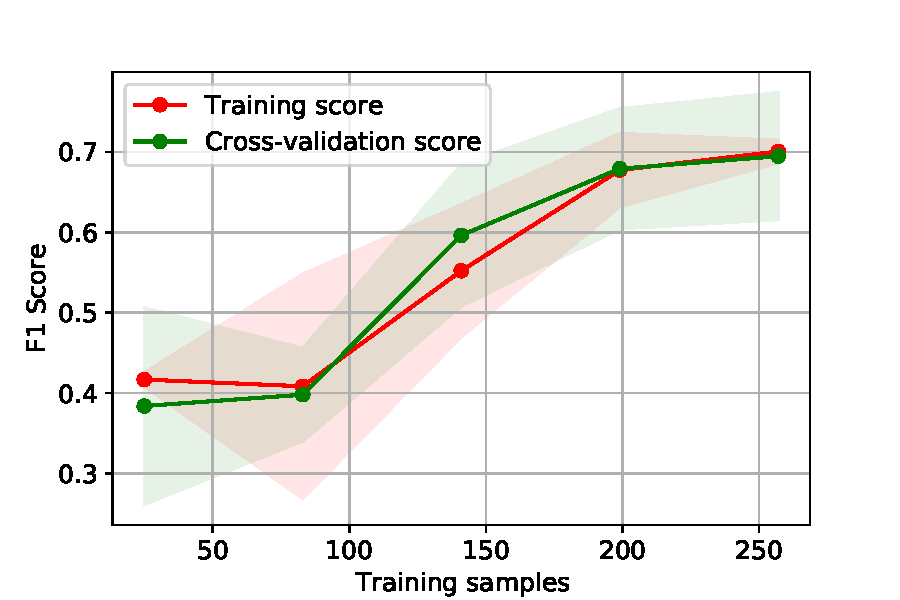
\includegraphics[width=8.5cm]{plots/SVM TVT LC F1.pdf}
\caption{Linear SVM Learning Curve}
\vspace{-0.5em}
\label{svmlc}
\centering
\end{figure}

For SVMs, the two main hyperparameters that were adjusted were the kernel type and penalty value $C$. Using a linear kernel was demonstrated to have the highest F1 score on the test set compared to other kernels, and $C$ was chosen to be 0.20. The learning curve for an SVM model using a linear kernel is shown in Figure \ref{svmlc}.